\section{Enigma und Turing Bombe}

\subsection{Historie}
Turing beschäftigte sich bereits vor Beginn des zweiten Weltkriegs mit den Enigma Maschinen, allerdings waren diese von den Italienern und wesentlich simpler wie die Enigma Maschinen später genutzt von den Deutschen. Die erste version der Enigma war frei verkäuflich und wurde eher private genutzt da sie nicht viel Sicherheit bat. In dieser version gab es lediglich 3 der in Sektion \ref{sec:rader} beschriebenen Räder, die in unterschiedlicher Reihenfolge eingesetzt werden konnten. Damit gab es lediglich $3! = 6$ Anordnungsmöglichkeiten. Zu dieser Zeit gab es außerdem kein, wie in Sektion \ref{sec:steck} aufgeführtes Steckbrett. Ein polnisches Verschlüsselungsteam unter der Leitung von Marian Rejewski legte den Grundstein und knackte die Verschlüsselungen der Enigma sehr schnell dort wurden sie zum ersten mal mit Steckbrett Versionen konfrontiert. Diese knackten sie von Hand mit Hilfe von Lochpapieren. Deutschland wollte sich diese Verschlüsselungsmaschinen nun für Militärische Zwecke zu nutzen machen, so entwickelten sie die nächste Version, die militärische Enigma. In dieser version wurden zwei Zahnräder zur Auswahl hinzugefügt. Nun wurden also 3 aus 5 Zahnrädern genommen und in unterschiedlichen Anordnungen in der Enigma kombiniert. Diese wurden nachher Großflächig für die deutsche Luftwaffe und Arme eingesetzt. Doch Marine war das nicht genug. Unter Admiral Karl Dönitz wurde eine Enigma Speziell für die Marine entwickelt bei der zu erst 3 aus 8 Zahnrädern und später dann 4 aus 8 Zahnrädern für die Verschlüsselung verwendet. Zu allem Überfluss drehten sich die Räder 6 bis 8 zweimal. Damit explodierten die Möglichen Kombinationen fast exponentiell. Bei Ausbruch des Krieges wurde Turing zusammen mit Neuntausend anderen Spezialisten in den Bletchley Park geholt. Dieser Park wurde zu einer wahren Entschlüsselungsfabrik, in dem später mit Hilfe der \emph{Bombe} 39 Tausend Enigma Nachrichten im Monat entschlüsselt wurden. Die sogenannte \emph{Bombe} war eine automatisierte Maschine zur Entschlüsselung der Enigma Nachrichten. Diese wurde ursprünglich von den Polen bis zur Invasion entwickelt. Durch die Invasion jedoch Übergaben sie die von den Polen \emph{Bomba} genannte Maschine an die Briten. Dort bauten sie die Maschine weiter aus und bauten im Zuge des Krieges zwischen 60 und 100 verschiedene \emph{Bombes} in Großbritannien und noch einmal mindestens so viel in der USA. Dort halfen sie dem Briten beim dechiffrieren per Unterseekabel. \cite{enigmaproblem1} \cite{theessentialturing}

\subsection{Enigma}
Die Enigma Maschine ist eine Verschlüsselungsmaschine, die im zweiten Weltkrieg von den Deutschen genutzt wurde. \\
Bestandteile der Enigma:
\begin{enumerate}
\item Eingabetastatur
\item beleuchtbare Anzeige
\item Steckbrett
\item Reflector
\item drei Zahnräder
\end{enumerate}

\subsubsection{Eingabetastatur}
Eine Schreibmaschienenähnliche Tastatur mit allen 26 Buchstaben des Alphabets, in die man die Nachricht eintippen konnte.

\subsubsection{beleuchtbare Anzeige}
Eine Anzeige mit allen 26 Buchstaben des Alphabets, die einzeln beleuchtet werden und die verschlüsselte Nachricht anzeigen z.B ein H wird eingetippt und ein R wird beleuchtet.

\subsubsection{Steckbrett}
\label{sec:steck}
Das Steckbrett, welches hinten an der Enigma Maschine angebracht war, diente zur Verschlüsselung, da man hier zehn von 26 Buchstaben manuell miteinander verlinken konnte. Somit wurde z.B. ein eingegebenes A zu einem H und anders herum.

\subsubsection{Zahnräder}
\label{sec:rader}
Die Zahnräder dienten zum weiteren Verschlüsseln der Nachrichten und jedes Zahnrad hatte 26 Stufen für jeden Buchstaben des Alphabets. Das Erste Zahnrad, welches die Eingabe passierte drehte sich bei jedem Tastendruck um einen Buchstaben weiter, das zweite Zahnrad mit jedem 26sten Tastendruck und das dritte bei jedem 676sten Tastendruck, also immer wenn das vorige Zahnrad sich einmal komplett gedreht hatte. Diese drei Zahnräder haben dadurch 17.576 (26 x 26 x 26) mögliche Kombinationen.

\subsubsection{Funktion}
Die Enigma Maschine konnte eine Nachricht in $10^{16}$ verschiedenen Weisen verschlüsseln.

\subsubsection{Beispiel}

\begin{figure}[hbtp]
\centering
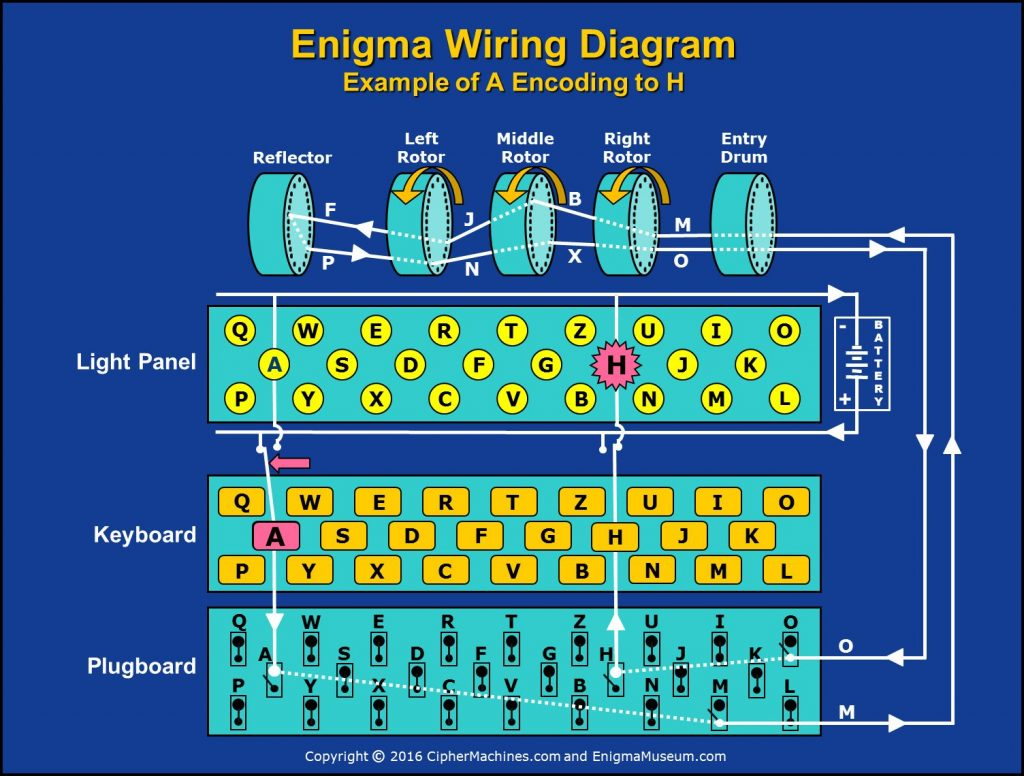
\includegraphics[scale=0.2]{Enigma_Maschine_Beispiel.jpg}
\caption{http://enigmamuseum.com/wp-content/uploads/2016/12/WiringDiagram-1024x776.jpg}
\end{figure}

Der eingegebene Buchstabe A geht erst einmal an das Steckbrett und ist hier mit dem Buchstaben M verbunden. Dieser wird dann an die Zahnräder weitergegeben, die den Buchstaben je nach Stellung verändern, hier von B zu J und schließlich F. Anschließend wird der Buchstabe wieder zurück durch die Zahnräder geleitet und kommt in diesem Beispiel als O heraus und wird wieder an das Steckbrett weitergeleitet. Der Buchstabe O ist hier mit H verbunden und so wird am Ende H in der Anzeige beleuchtet, und somit wurde A zu H verschlüsselt.

\subsection{Turing Bombe}


\subsection{(Bamboo Technik)?}